\chapter{Correlation of \diiid's toroidally separated interferometers}
\label{ch:ToroidalCorrelation}
The toroidal structure of an MHD mode can have important implications
for the mode's stability and its interaction with the surrounding plasma.
A mode's toroidal structure is typically characterized
by its toroidal mode number $n$.
Historically, measurement of toroidal (and poloidal) mode numbers
with external magnetic probes has provided rich insight
into the physics governing numerous operational regimes and stability limits.
However, core-localized MHD produces weak signals outside of the plasma volume,
making measurement of the corresponding mode numbers
via external magnetic probes difficult or impossible.
Recently, measurements from toroidally separated
electron cyclotron emission imaging (ECEI) systems
on the KSTAR tokamak have identified mode numbers of
sawteeth~\cite{choe_nf_2015},
demonstrating the utility of using more exotic measurements
to probe the structure of core-localized MHD.

This chapter describes the correlation
of toroidally separated interferometers
to measure toroidal mode numbers.
To the author's knowledge,
this is the first such implementation in a tokamak.
As the interferometers are capable of probing the plasma core,
their correlation allows direct measurement
of the toroidal structure of core-localized modes
--- a long-sought after and first-of-its-kind measurement at \diiid.
Below, Section~\ref{sec:ToroidalCorrelation:TwoPointCorrelation}
reviews the two-point correlation technique,
which allows inference of a propagating wave's
spatial structure from measurements
made at two distinct spatial locations.
Section~\ref{sec:ToroidalCorrelation:Interferometers}
then examines the geometry of the interferometers and
develops a formula for the measured toroidal mode number.
Section~\ref{sec:ToroidalCorrelation:ImplementationDetails}
describes the careful efforts to eliminate timebase discrepancies
between the two interferometer systems,
validates the interferometer-measured toroidal mode numbers
against those measured by external magnetic probes, and
discusses the effect of the interferometers' radial offset.
Finally, Section~\ref{sec:ToroidalCorrelation:CoreLocalized}
provides an encouraging proof of principle
regarding the ability of the correlated interferometers
to diagnose core-localized MHD.


\section{Two-point correlation}
\label{sec:ToroidalCorrelation:TwoPointCorrelation}
Two-point correlation allows inference
of a propagating wave's spatial structure
from measurements made at two distinct spatial locations.
Below,
Section~\ref{sec:ToroidalCorrelation:TwoPointCorrelation:wavenumber_measurement}
details the two-point correlation technique.
Section~\ref{sec:ToroidalCorrelation:TwoPointCorrelation:aliasing}
then discusses the aliasing of large wavenumbers and
establishes a measurement's Nyquist wavenumber,
below which wavenumbers are \emph{not} aliased.
Finally,
Section~\ref{sec:ToroidalCorrelation:TwoPointCorrelation:toroidal_mode_numbers}
converts the results of the previous sections
into their toroidal-mode-number equivalents,
as is conventional for fluctuation characterization in a tokamak.


\subsection{Wavenumber measurement via two-point correlation}
\label{sec:ToroidalCorrelation:TwoPointCorrelation:wavenumber_measurement}
Consider a $1$-dimensional, coherent density fluctuation
with amplitude $\tilde{n}_0$, wavenumber $k$, and angular frequency $\omega$
\begin{equation}
  \tilde{n}(z, t)
  =
  \tilde{n}_0
  e^{i(k z - \omega t)}.
  \label{eq:ToroidalCorrelation:coherent_density_fluctuation}
\end{equation}
Imagine that the density is measured
at two locations separated by distance $\Delta z$,
producing two time series, $x(t)$ and $y(t)$, given as
\begin{align}
  x(t)
  &=
  \tilde{n}(z_0, t)
  \\
  y(t)
  &=
  \tilde{n}(z_0 + \Delta z, t)
  =
  x(t) e^{i k \Delta z}.
\end{align}
The cross phase $\alpha_{xy}$ between these two time series is
\begin{align}
  \alpha_{xy}
  &=
  \arg\left[ x^*(t) \cdot y(t) \right]
  \label{eq:ToroidalCorrelation:cross_phase}
  \\
  &=
  k \Delta z,
\end{align}
where $x^*$ is the complex conjugate of $x$.
Thus, a measured wavenumber $k_{\meas}$
can be inferred from the cross phase via
\begin{equation}
  k_{\meas} = \frac{\alpha_{xy}}{\Delta z}.
  \label{eq:ToroidalCorrelation:wavenumber_from_cross_phase}
\end{equation}
The cross phase $\alpha_{xy}$ of $x(t)$ and $y(t)$
can be readily estimated via
the non-parametric, FFT-based
spectral-estimation techniques discussed in
Appendix~\ref{app:SpectralEstimation:NonParametric}.
Note that such cross-phase estimates are frequency-resolved,
allowing simultaneous characterization
of multiple fluctuations at distinct frequencies.


\subsection{Aliasing \& the Nyquist wavenumber}
\label{sec:ToroidalCorrelation:TwoPointCorrelation:aliasing}
The measured wavenumber
(\ref{eq:ToroidalCorrelation:wavenumber_from_cross_phase})
may be \emph{aliased}.
To see this, note that the cross-phase estimate $\alpha_{xy}$
is only unique modulo $2 \pi$
(that is, $0$ is equivalent to $\pm 2 \pi$, $\pm 4 \pi$, etc.).
If the fluctuation wavenumber $k$ is sufficiently large
(i.e.\ if it exceeds the so-called Nyquist wavenumber $k_{\Ny}$),
this cross-phase ambiguity aliases the measured wavenumber
(\ref{eq:ToroidalCorrelation:wavenumber_from_cross_phase})
away from the true wavenumber.

In the most general case,
the wave's propagation direction is not known \emph{a priori}, and
both positive and negative wavenumbers should be considered
(i.e.\ $-\pi < \alpha_{xy} \leq \pi$).
This cross-phase domain yields a Nyquist wavenumber
\begin{equation}
  k_{\Ny} = \frac{\pi}{\Delta z},
  \qquad \text{for \emph{unknown} propagation direction.}
  \label{eq:ToroidalCorrelation:Nyquist_wavenumber_unknown_propagation}
\end{equation}
Wavenumber measurements
(\ref{eq:ToroidalCorrelation:wavenumber_from_cross_phase})
from fluctuations with $|k| > k_{\Ny}$ are aliased, while
measurements from fluctuations with $|k| \leq k_{\Ny}$ are not aliased.
Note that
(\ref{eq:ToroidalCorrelation:Nyquist_wavenumber_unknown_propagation})
is equivalent to the famed Nyquist frequency:
making the transformations $\Delta z \rightarrow 1 / f_s$
for temporal sampling rate $f_s$ and
$k \rightarrow 2 \pi f$,
(\ref{eq:ToroidalCorrelation:Nyquist_wavenumber_unknown_propagation})
readily becomes $f_{\Ny} = f_s / 2$.
Thus, $1 / \Delta z$ can be thought of as the spatial sampling rate,
with a larger sampling rate (i.e.\ smaller $\Delta z$)
allowing un-aliased measurements of larger wavenumbers.

Now, if the wave's propagation direction is known \emph{a priori}
(for example, if the wave propagation is dominated by advection, and
the fluid velocity is well-diagnosed),
only a single polarity of wavenumbers need to be considered.
For concreteness, positive wavenumbers are considered below
(i.e.\ $0 \leq \alpha_{xy} < 2 \pi$).
This cross-phase domain yields a Nyquist wavenumber
\begin{equation}
  k_{\Ny} = \frac{2 \pi}{\Delta z},
  \qquad \text{for \emph{known} propagation direction.}
  \label{eq:ToroidalCorrelation:Nyquist_wavenumber_known_propagation}
\end{equation}


\subsection{Measurement of toroidal mode numbers}
\label{sec:ToroidalCorrelation:TwoPointCorrelation:toroidal_mode_numbers}
Fluctuations in a torus are often characterized
by their toroidal $n$ and poloidal $m$ mode numbers,
both of which are constrained to be integers
by the toroidal and poloidal periodicities, respectively, of the torus.
For a torus with major radius $R$,
the toroidal mode number $n$ is related
to the toroidal wavenumber $k_{\zeta}$ as
\begin{equation}
  k_{\zeta} = \frac{n}{R},
\end{equation}
and the toroidal angular separation $\Delta \zeta$
is related to the spatial separation $\Delta z$ as
\begin{equation}
  \Delta \zeta = \frac{\Delta z}{R}.
\end{equation}
Using these definitions,
the above formulas for the measured wavenumber and the Nyquist wavenumber
can be rewritten in terms of toroidal mode numbers as follows:
\begin{align}
  n_{\text{meas}}
  &=
  \frac{\alpha_{xy}}{\Delta \zeta},
  \label{eq:ToroidalCorrelation:modenumber_from_cross_phase}
  \\
  n_{\text{Ny}}
  &=
  \begin{cases}
    \frac{\pi}{\Delta \zeta}
    \qquad \text{for \emph{unknown} propagation direction} \\
    \frac{2 \pi}{\Delta \zeta}
    \qquad \text{for \emph{known} propagation direction}
  \end{cases}.
  \label{eq:ToroidalCorrelation:Nyquist_modenumber}
\end{align}


\section{Toroidal correlation of interferometers}
\label{sec:ToroidalCorrelation:Interferometers}
This section applies two-point correlation
to the measurement of toroidal mode numbers
with \diiid's toroidally separated, heterodyne CO$_2$ interferometers.
Section~\ref{sec:ToroidalCorrelation:Interferometers:diiid}
describes the geometry of the interferometer probe beams,
which establishes the Nyquist toroidal mode number.
Sections~\ref{sec:ToroidalCorrelation:Interferometers:phase_fluctuations} and
\ref{sec:ToroidalCorrelation:Interferometers:interferometer_measured_mode_number}
then examine the relationship between
the interferometer-measured phase fluctuations and
the toroidal mode number.
As the interferometers are capable of probing the plasma core,
their correlation allows direct measurement
of the toroidal structure of core-localized modes
--- a long-sought after and first-of-its-kind measurement at \diiid.


\subsection{\diiid's interferometers}
\label{sec:ToroidalCorrelation:Interferometers:diiid}
\diiid's multichannel, two-color, heterodyne CO$_2$ interferometer
measures both the equilibrium~\cite{carlstrom_rsi88} and
fluctuating~\cite{vanzeeland_ppcf05, pace_nf17} components
of the line-integrated electron density.
Each channel is configured as a Michelson interferometer,
with each probe beam making a double-pass through the plasma.
The three vertical chords pass through the $V1$, $V2$, and $V3$ ports
at a toroidal location of $240^{\circ}$, while
the radial chord passes through the $R0$ port
at a toroidal location of $225^{\circ}$.
Of particular relevance to this work is the $V2$ interferometer,
which has a major-radial location $R = \SI{1.94}{\meter}$ and
is shown in Figure~\ref{fig:ToroidalCorrelation:pci_interf_locs}.
The viewing geometry influences
an interferometer's sensitivity to various MHD instabilities;
for example, vertical chords are more sensitive to
toroidal Alfv\'{e}n eigenmodes (TAEs), while
radial chords are more sensitive to
reversed-shear Alfv\'{e}n eigenmodes (RSAEs)
\cite{vanzeeland_ppcf05}.

\begin{figure}
  \centering
  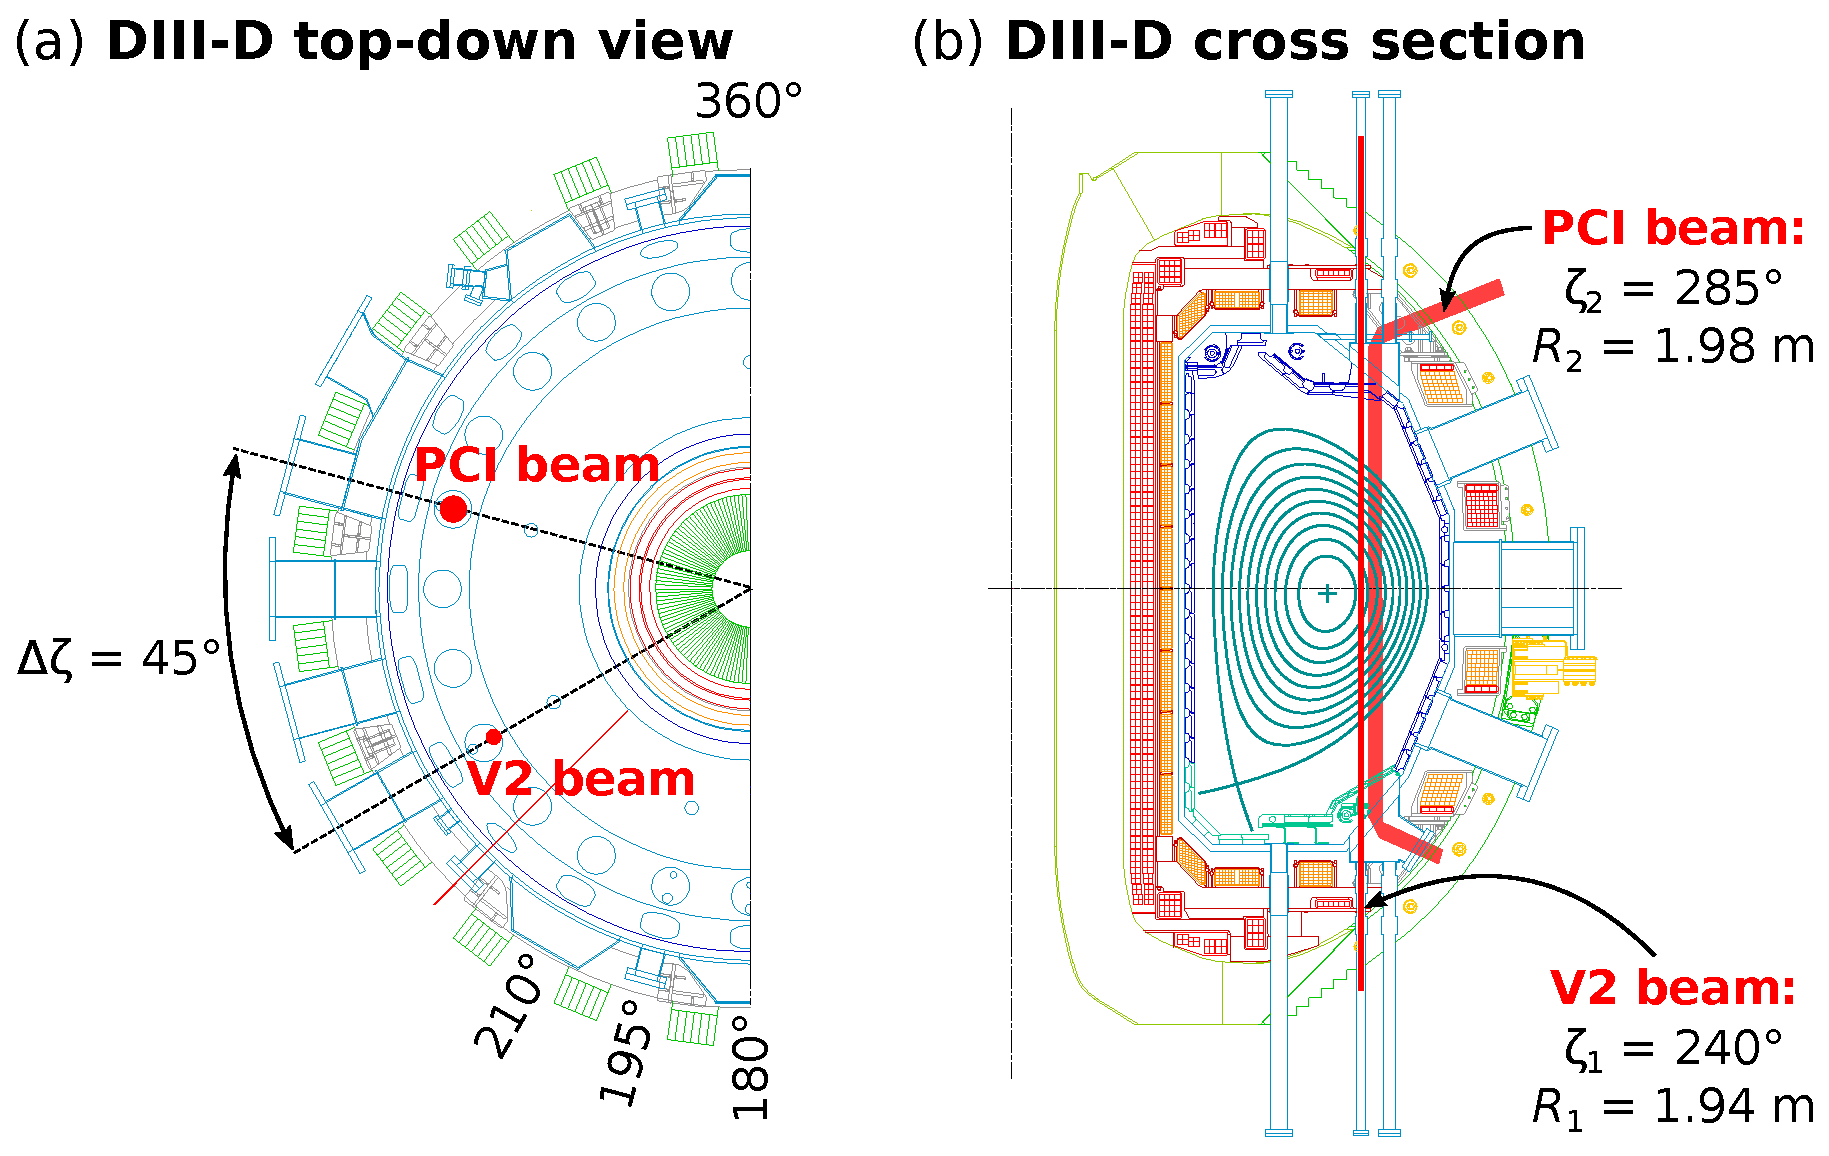
\includegraphics[width = \textwidth]{%
    Chapters/ToroidalCorrelation/figs/pci_interf_locs.pdf}
  \caption[Locations of the $V2$ and PCI interferometer beams on \diiid]{%
    (a) A top-down view of the \diiid\space vessel.
    The toroidal location of the $V2$ interferometer beam
    is $\zeta = 240^{\circ}$,
    and the toroidal location of the PCI beam
    is $\zeta = 285^{\circ}$.
    The \diiid\space sign convention for toroidal mode numbers
    is that $n > 0$ for modes that rotate counterclockwise
    when viewing the torus from above,
    as this corresponds to the direction of dominant torque injection.
    (b) A poloidal cross section of the \diiid\space vessel.
    The major-radial location of the $V2$ interferometer beam
    is $R = \SI{1.94}{\meter}$, and
    the major-radial location of the PCI beam
    is $R = \SI{1.98}{\meter}$.}
\label{fig:ToroidalCorrelation:pci_interf_locs}
\end{figure}

The addition of a heterodyne-interferometer channel
to \diiid's pre-existing phase contrast imaging (PCI) system
is discussed extensively in
Chapter~\ref{ch:Implementation} and
elsewhere~\cite{davis_rsi16}, but
the details of relevance to the toroidal-correlation measurement
are briefly reviewed here.
The PCI probe beam sits at a toroidal location of $285^{\circ}$ and
has a major-radial location $R = \SI{1.98}{\meter}$.
The location of the PCI beampath relative to that of the $V2$ interferometer
is shown in Figure~\ref{fig:ToroidalCorrelation:pci_interf_locs}.

The geometry of the $V2$ and PCI interferometers
has consequences for the toroidal-correlation measurement.
The interferometers are
toroidally spaced by $\Delta \zeta = 45^{\circ}$
such that the Nyquist toroidal mode number
(\ref{eq:ToroidalCorrelation:Nyquist_modenumber}) becomes
\begin{equation}
  n_{\text{Ny}}
  =
  \begin{cases}
    4
    \qquad \text{for \emph{unknown} propagation direction} \\
    8
    \qquad \text{for \emph{known} propagation direction}
  \end{cases}.
  \label{eq:ToroidalCorrelation:Nyquist_modenumber_interferometers}
\end{equation}
The \diiid\space sign convention for toroidal mode numbers
is indicated in Figure~\ref{fig:ToroidalCorrelation:pci_interf_locs};
that is, $n > 0$ for modes that rotate counterclockwise
when viewing the torus from above,
as this corresponds to the direction of dominant torque injection.
Consistency with this sign convention requires
that $x(t)$ corresponds to the $V2$ interferometer signal and
that $y(t)$ corresponds to the PCI interferometer signal
when computing the toroidal mode number via
(\ref{eq:ToroidalCorrelation:modenumber_from_cross_phase}).
Finally, the $V2$ and PCI interferometer beam paths have a slight radial offset
($\Delta R = \SI{4}{\centi\meter}$ with
$R_{\text{v2}} = \SI{1.94}{\meter}$ and
$R_{\text{pci}} = \SI{1.98}{\meter}$);
the consequences of this offset are discussed in
Section~\ref{sec:ToroidalCorrelation:ImplementationDetails:radial_offset}.

For completeness, it should also be mentioned that
a three-chord, radially viewing Faraday-effect polarimeter-interferometer
was recently installed on \diiid's $285^{\circ}$ $R0$ port~\cite{chen_rsi16}.
While diagnosing core-localized magnetic fluctuations
is the primary impetus for this installation,
the system also measures line-integrated electron-density fluctuations.
Presumably, these measurements could be correlated with those from
the $225^{\circ}$ $R0$ CO$_2$ heterodyne interferometer.
However, these two systems do not have phase-locked sampling rates
(the necessity of which is discussed in
Section~\ref{sec:ToroidalCorrelation:ImplementationDetails:phase_locked_sampling}),
so no attempts to correlate their interferometric measurements
are performed in this work.


\subsection{Interferometer-measured phase fluctuations}
\label{sec:ToroidalCorrelation:Interferometers:phase_fluctuations}
Consider a tokamak electron density fluctuation with
amplitude $\tilde{n}_0(r)$,
toroidal mode number $n$,
poloidal mode number $m$, and
angular frequency $\omega$
\begin{equation}
  \tilde{n}_e(\vect{r}, t)
  =
  \tilde{n}_0(r)
  e^{i \left(n \zeta + m \theta - \omega t \right)}.
\end{equation}
The phase fluctuation (\ref{eq:InterferometricMethods:phase_fluctuation})
imparted to a CO$_2$ probe beam
propagating \emph{vertically} through $\tilde{n}_e(\vect{r}, t)$ becomes
\begin{align}
  \tilde{\phi}
  &=
  - r_e \lambda_0 \int \tilde{n}_e(\vect{r}, t) dz.
  \notag \\
  &=
  \Phi e^{i \left( n \zeta - \omega t \right)},
  \label{eq:ToroidalCorrelation:phase_fluctuations_vertical_beam1}
\end{align}
where
\begin{equation}
  \Phi
  =
  -r_e \lambda_0
  \int \tilde{n}_0(r) e^{i m \theta} dz
  \label{eq:ToroidalCorrelation:line_integrated_radial_and_poloidal_structure}
\end{equation}
is a complex-valued function of
the beam's major-radial location and
the radial and poloidal mode structure.
For a given mode,
the $V2$ and PCI interferometers see the same
radial and poloidal mode structure such that
$\Phi$ effectively reduces to a one-dimensional function $\Phi = \Phi(R)$.
Further, $\Phi$ can be written explicitly
as a complex value $\Phi = |\Phi| e^{i \sigma}$.
Thus, the phase fluctuation
(\ref{eq:ToroidalCorrelation:phase_fluctuations_vertical_beam1})
can be written alternatively as
\begin{equation}
  \tilde{\phi}
  =
  |\Phi(R)| e^{i[n \zeta - \omega t + \sigma(R)]},
  \label{eq:ToroidalCorrelation:phase_fluctuations_vertical_beam2}
\end{equation}
where the dependence on the major radius $R$ of the beam
has been noted explicitly.


\subsection{Interferometer-measured toroidal mode number}
\label{sec:ToroidalCorrelation:Interferometers:interferometer_measured_mode_number}
Define $x(t)$ and $y(t)$ to be
the $V2$-measured and PCI-measured phase fluctuations, respectively; i.e.\
\begin{align}
  x(t)
  &=
  \tilde{\phi}_{\text{v2}}(t)
  =
  |\Phi(R_{\text{v2}})|
  e^{i[n \zeta_{\text{v2}} - \omega t + \sigma(R_{\text{v2}})]},
  \\
  y(t)
  &=
  \tilde{\phi}_{\text{pci}}(t)
  =
  |\Phi(R_{\text{pci}})|
  e^{i[n \zeta_{\text{pci}} - \omega t + \sigma(R_{\text{pci}})]}.
\end{align}
Then the cross phase (\ref{eq:ToroidalCorrelation:cross_phase}) becomes
\begin{equation}
  \alpha_{xy}
  =
  n \Delta \zeta
  +
  \left[%
    \sigma(R_{\text{pci}})
    -
    \sigma(R_{\text{v2}})
  \right],
  \label{eq:ToroidalCorrelation:interferometer_measured_cross_phase}
\end{equation}
where $\Delta \zeta = \zeta_{\text{pci}} - \zeta_{\text{v2}} = 45^{\circ}$
is the toroidal separation between the interferometer beams.
The cross phase $\alpha_{xy}$ of $x(t)$ and $y(t)$
can be readily estimated via
the non-parametric, FFT-based
spectral-estimation techniques discussed in
Appendix~\ref{app:SpectralEstimation:NonParametric}, but
$\sigma(R_{\text{pci}})$ and $\sigma(R_{\text{v2}})$
are not typically known \emph{a priori}.
Nonetheless, the measured toroidal mode number $n_{\meas}$ is defined as
\begin{equation}
  n_{\meas}
  =
  \frac{\alpha_{xy}}{\Delta \zeta},
  \qquad
  \text{where} \;\, \Delta \zeta = 45^{\circ}.
  \label{eq:ToroidalCorrelation:interferometer_measured_mode_number}
\end{equation}
However, if $\sigma(R_{\text{pci}}) \neq \sigma(R_{\text{v2}})$,
the measured mode number will not be equal to the true mode number
(i.e.\ $n_{\meas} \neq n$);
this is discussed further in
Section~\ref{sec:ToroidalCorrelation:ImplementationDetails:radial_offset}.
Further, if the true mode number exceeds the Nyquist mode number
(\ref{eq:ToroidalCorrelation:Nyquist_modenumber_interferometers}),
the measured mode number will be aliased away from the true mode number
(i.e.\ $n_{\meas} \neq n$).


% \subsection{MHD plasma-density perturbations}
% \label{sec:ToroidalCorrelation:Interferometers:MHD_theory}
% An MHD mode displaces a plasma from it's equilibrium position
% by $\vect{\xi} = \vect{\xi}(\vect{r}, t)$.
% The perturbed velocity is given as
% $\vect{v}_1 = \partial \vect{\xi} / \partial t$
% and, assuming harmonic variations, reduces to
% \begin{equation}
%   \vect{v}_1
%   \equiv
%   \frac{\partial \vect{\xi}}{\partial t}
%   =
%   -i \omega \vect{\xi},
%   \notag
% \end{equation}
% where $\omega$ is the mode's angular frequency.
% The plasma density $n_i$ is given as
% \begin{equation}
%   n_i = \bar{n}_i + \tilde{n}_i,
%   \notag
% \end{equation}
% where $\bar{n}_i$ and $\tilde{n}_i$ are
% the equilibrium and fluctuating components, respectively.
% Assuming a stationary equilibrium ($\vect{v}_0 = 0$) and
% using the above relations,
% the linearized continuity equation reduces to
% \begin{equation}
%   \tilde{n}_i = -\nabla \cdot (\bar{n}_i \vect{\xi}).
%   \label{eq:ToroidalCorrelation:density_fluctuations}
% \end{equation}
% If we relax the assumption on $\vect{v}_0$ to allow
% finite equilibrium flow ($\vect{v}_0 \neq 0$),
% then the right-hand side of (\ref{eq:ToroidalCorrelation:density_fluctuations})
% is simply multiplied by the prefactor
% $[1
% - (\vect{v}_0 \cdot \vect{k} / \omega)
% + i (\nabla \cdot \vect{v}_0 / \omega)]^{-1}$, where
% $\vect{k}$ is the mode wavevector.


\section{Implementation details and non-ideal effects}
\label{sec:ToroidalCorrelation:ImplementationDetails}
This section discusses various implementation details and non-ideal effects
regarding the toroidal correlation of the $V2$ and PCI interferometers.
Specifically, Section~\ref{sec:ToroidalCorrelation:ImplementationDetails:phase_locked_sampling}
describes the modifications to the $V2$ and PCI digitizers
that now enable phase-locked measurements.
Section~\ref{sec:ToroidalCorrelation:ImplementationDetails:trigger_offset}
unveils the presence of a deleterious ``trigger offset''
between the phase-locked systems but
also demonstrates an easy and robust methodology
for estimating and compensating this offset
in post-processing software.
Section~\ref{sec:ToroidalCorrelation:ImplementationDetails:validation_agains_magnetics}
then compares the interferometer-measured toroidal mode numbers
with those measured by \diiid's array of midplane magnetic probes,
typically resulting in good agreement for large, robust tearing modes.
Finally, Section~\ref{sec:ToroidalCorrelation:ImplementationDetails:radial_offset}
discusses how the $\Delta R = \SI{4}{\centi\meter}$ major-radial offset
between the $V2$ and PCI interferometers
can bias the measured toroidal mode numbers;
eliminating this radial offset is not possible
with the current port allocations, but
future work to empirically or computationally account
for the radial and poloidal mode structures
may aid the interpretation
of the interferometer-measured toroidal mode numbers.


\subsection{Phase-locked sampling}
\label{sec:ToroidalCorrelation:ImplementationDetails:phase_locked_sampling}
Extracting useful information
from the correlation of two measurements
requires that the sampling rates of the two measurements
are \emph{phase-locked}.
If the sampling rates are \emph{not} phase-locked,
slippage between the sampling times
will result in artificial evolution of the measured phase.

Digitizing the two signals on a common digitizer
is the simplest method for ensuring phase-locked sampling.
Unfortunately, such an approach is not suitable
for the $V2$ and PCI interferometer signals.
The $V2$ interferometer's
$\Delta f_0 = \SI{40}{\mega\hertz}$ intermediate-frequency signal
is demodulated using an all-digital technique
that mandates use of a sampling rate
$f_s = (4 / 3) \Delta f_0$
\cite{vanzeeland_rsi08}, and
the baseband $I$ and $Q$ signals never exist in analog form.
In contrast, as described in
Chapter~\ref{ch:Implementation} and \cite{davis_rsi16},
the PCI interferometer's
$\Delta f_0 = \SI{30}{\mega\hertz}$ intermediate-frequency signal
is demodulated with analog electronics, and
the analog baseband $I$ and $Q$ signals
are then digitized on two channels of a D-tAcq ACQ$216$ CPCI board.
Because the $V2$ interferometer's baseband $I$ and $Q$ signals
never exist in analog form,
it is not possible to digitize the $V2$ $I$ and $Q$ signals
on the digitizer used by the PCI interferometer.
Further, because of the intermediate-frequency mismatch
between the $V2$ and PCI interferometers,
it is also not possible digitally demodulate and digitize
the PCI interferometer's $\SI{30}{\mega\hertz}$ intermediate-frequency signal
using the $V2$ interferometer's
$\SI{40}{\mega\hertz}$ digital demodulation system.
An alternative approach is to directly digitize
both intermediate-frequency signals
with a high-bandwidth digitizer and
demodulate both signals in software,
as has been done elsewhere~\cite{mlynek_fst12}.
While \diiid's ion cyclotron emission (ICE) digitizer
has a $200 \, \text{MSPS}$ sample rate,
channels on the ICE digitizer are not consistently available.

As sharing a common digitizer is not possible,
phase-locked sampling between the $V2$ and PCI interferometers
requires that the digitizers of both systems
derive their clocks from a common source.
The $V2$ interferometer derives its clock
from a $\SI{320}{\mega\hertz}$ oven-controlled crystal oscillator (OCXO), and
its digital demodulation system
has two auxiliary outputs that can be programmed
to output phase-locked LVCMOS signals
at $\SI{320}{\mega\hertz} / N$, where
$N \in \{1, 2, 3, ..., 32\}$.
Both outputs are currently programmed with divisor $N = 20$
such that they each provide a $\SI{16}{\mega\hertz}$ clock signal.
One of these $\SI{16}{\mega\hertz}$ clock signals
is routed via an RG-$58$ coaxial cable
from the $V2$ digital demodulation hardware
in the first row of the \diiid\space annex
to the PCI digitizer
in the third row of the \diiid\space annex.

The PCI digitizer typically samples at $f_s = 4 \, \text{MSPS}$.
Thus, division of the $V2$ $\SI{16}{\mega\hertz}$ clock by four
(in hardware or software) yields a clock appropriate for typical sampling.
Each board of the PCI digitizer can accept an external clock
through the front panel's single-pin LEMO CLK input.
The CLK signal passes through an optocoupler
with a bandwidth $\sim \SI{10}{\mega\hertz}$
\cite{milne_optocoupler_pc16}, but
in-house tests have demonstrated
that the input clock frequency
can actually exceed $\SI{16}{\mega\hertz}$.
As a result, the $\SI{16}{\mega\hertz}$ signal
is directly connected to the front-panel LEMO CLK input
of the ``master'' digitizer board (``board $8$''), and
the necessary division
(i.e.\ divide by four to achieve typical $4 \, \text{MSPS}$ sampling rate)
is performed within the digitizer board,
which is cleaner, simpler, and more easily extensible
than performing the division in hardware.
The resulting $\SI{4}{\mega\hertz}$ clock
is routed to the ``slave'' digitizer board (``board $7$'')
via the PXI backplane.
The phase-locked sampling of the $V2$ and PCI systems
has been in place since June 2016.


\subsection{Estimating \& compensating the ``trigger offset''}
\label{sec:ToroidalCorrelation:ImplementationDetails:trigger_offset}
As discussed in Appendix~\ref{app:DigitizerSynchronization},
phase-locked digitizers can still suffer from
a so-called ``trigger offset'', as defined by
(\ref{eq:DigitizerSynchronization:trigger_offset}).
A finite trigger offset results
(a) when a digitizer triggers at a time $\delta t$ later
than its nominal trigger time and
(b) when the sampling rate deviates from the nominal sampling rate
and the nominal trigger times of both digitizers differ.

A finite trigger offset biases mode-number measurements.
For example, Figure~\ref{fig:ToroidalCorrelation:trigger_offset}(a)
displays the toroidal mode numbers of two coherent modes
as measured by the uncompensated interferometers.
Note that the measured mode number of each mode
(unphysically) evolves with the mode frequency,
which is consistent
(see (\ref{eq:DigitizerSynchronization:measured_phase_difference}))
with the presence of a finite trigger offset
between the interferometer measurements.
Referencing
(\ref{eq:DigitizerSynchronization:trigger_offset_estimate_frequency_swept}),
the trigger offset can be estimated
from the measured mode-number evolution
during a linear frequency sweep as
\begin{align}
  \delta t_{\trig}
  =
  \frac{d \alpha_{xy}}{d\omega}
  \approx
  \frac{\Delta \alpha_{xy}}{\Delta \omega}
  \approx
  \SI{30}{\micro\second},
\end{align}
where
$\Delta \alpha_{xy} = \Delta \zeta \cdot \Delta n_{\meas}$
is the measured phase-angle change and
$\Delta \zeta = \pi / 4$
is the angular separation of the interferometers
(consistent with
(\ref{eq:ToroidalCorrelation:interferometer_measured_mode_number}));
here, the numerical value results from
$\Delta n_{\meas} \approx 5$ and
$\Delta \omega \approx 2 \pi \cdot \SI{20}{\kilo\hertz}$,
as indicated by the red circular annotations
to the lower-frequency mode in
Figure~\ref{fig:ToroidalCorrelation:trigger_offset}(a).
Note that $\delta t_{\trig} > 0$
implies that the actual sampling times
of the PCI interferometer lag (i.e.\ occur later than)
those of the $V2$ interferometer, as shown schematically in
Figure~\ref{fig:DigitizerSynchronization:trigger_offset_schematic}.
Applying standard techniques~\cite[Sec.~4.5]{oppenheim}
in post-processing software
to eliminate this $\SI{30}{\micro\second}$ timebase discrepancy
dramatically reduces the unphysical mode-number evolution observed in
Figure~\ref{fig:ToroidalCorrelation:trigger_offset}(a).
Scanning $\delta t_{\trig}$ about $\SI{30}{\micro\second}$
shows that the unphysical mode-number evolution is minimized for
\begin{equation}
  \delta t_{\trig}
  =
  \SI{32.5}{\micro\second}.
  \label{eq:ToroidalCorrelation:trigger_offset_optimized}
\end{equation}
Figure~\ref{fig:ToroidalCorrelation:trigger_offset}(b)
displays the interferometer-measured toroidal mode numbers
after compensating for trigger offset
(\ref{eq:ToroidalCorrelation:trigger_offset_optimized});
note that the mode numbers are constant in time,
consistent with physical expectations.
It should be emphasized that the only difference between
Figure~\ref{fig:ToroidalCorrelation:trigger_offset}(a) and
Figure~\ref{fig:ToroidalCorrelation:trigger_offset}(b)
is the compensation of trigger offset
(\ref{eq:ToroidalCorrelation:trigger_offset_optimized}).

\begin{figure}
  \centering
  \includegraphics[width = \textwidth]{%
    Chapters/ToroidalCorrelation/figs/trigger_offset.pdf}
  \caption[``Trigger offset'' compensation]{%
    Interferometer-measured toroidal mode numbers
    (a) \emph{without} compensation for the trigger offset and
    (b) \emph{with} compensation for the trigger offset.
    In (a), the finite trigger offset
    (\ref{eq:ToroidalCorrelation:trigger_offset_optimized})
    results in the unphysical evolution
    of the measured toroidal mode numbers.
    The trigger offset is roughly estimated
    from the measured mode-number evolution
    between the red circular annotations
    to the lower-frequency mode
    ($\Delta f \approx \SI{20}{\kilo\hertz}$ and
    $\Delta n \approx 5$; note that $\Delta n_{\meas}$
    refers to the total number of mode numbers evolved through,
    i.e.\ it is path-dependent and is \emph{not} simply
    the difference between the final and initial $n_{\meas}$).
    In (b), the digital records of both interferometers
    have been synchronized by compensating for the finite trigger offset
    (\ref{eq:ToroidalCorrelation:trigger_offset_optimized}), and
    the measured toroidal mode numbers are constant in time,
    consistent with physical expectations.
    The $6$-digit number in the upper right-hand corner
    indicates the \diiid\space shot.
  }
\label{fig:ToroidalCorrelation:trigger_offset}
\end{figure}

Trigger offset (\ref{eq:ToroidalCorrelation:trigger_offset_optimized})
has been robustly stable
since phase-locking the $V2$ and PCI digitizers in June 2016,
a timescale currently exceeding one year.
It is interesting to examine the physical origin
of this trigger offset to understand when it might change.
Referencing the definition of $\delta t_{\trig}$ in
(\ref{eq:DigitizerSynchronization:trigger_offset}),
there are three distinct mechanisms contributing to the trigger offset.
The first effect is the difference
between the trigger-time discrepancies $\delta t_j$ of each digitizer;
in a properly functioning digitizer,
this is discrepancy is typically smaller than one or two sample times
(i.e.\ $\lesssim \SI{1}{\micro\second}$ for the digitizers considered here),
making it an unlikely source of the relatively large trigger offset
(\ref{eq:ToroidalCorrelation:trigger_offset_optimized}).
The second effect is
the digitizers' normalized sampling-rate deviation $\bar{\delta F_j}$
(phase-locked digitizers have \emph{equal}
normalized sampling-rate deviations;
see (\ref{eq:DigitizerSynchronization:phase_locked_normalized_sample_rate_deviations})).
Because the trigger offset
(\ref{eq:ToroidalCorrelation:trigger_offset_optimized})
does \emph{not} appear to vary in time,
temporal fluctuations in $\bar{\delta F_j}$ cannot be responsible;
however, $\bar{\delta F_j}$ will be constant and finite
if the sampling rate has a constant offset
from the nominal sampling rate.
The third effect is the weighting of $\bar{\delta F_j}$
by the difference in nominal trigger times.
Now, the $V2$ digitizer nominally triggers at
$t_{\text{v2}}^{\nom}[0] \approx \SI{-1.5}{\second}$
relative to plasma breakdown, while
the PCI digitizer nominally triggers at
$t_{\text{pci}}^{\nom}[0] = \SI{-0.05}{\second}$
relative to plasma breakdown.
Solving for the $\bar{\delta F_j}$ in
(\ref{eq:DigitizerSynchronization:trigger_offset}) and
neglecting the small trigger-time discrepancies $\delta t_j$ yields
\begin{equation}
  \bar{\delta F_j}
  \approx
  \frac{\delta t_{\trig}}{t_{\text{pci}}^{\nom}[0] - t_{\text{v2}}^{\nom}[0]}
  \approx
  2.2 \times 10^{-5},
\end{equation}
which is not an unreasonable precision
for the digitizer sampling rates.
Thus, digitizer offset
(\ref{eq:ToroidalCorrelation:trigger_offset_optimized})
appears to result from the combined effects of
finite sampling-rate precision (i.e.\ nonzero $\bar{\delta F_j}$) and
the difference between the nominal trigger times
of the $V2$ and PCI digitizers.
Importantly, if the nominal trigger times of
the $V2$ or PCI digitizers are altered in the future,
the trigger offset will also change and
will need to be estimated from new measurements.


\subsection{Validation against magnetic measurements}
\label{sec:ToroidalCorrelation:ImplementationDetails:validation_agains_magnetics}
\begin{figure}
  \centering
  \includegraphics[width = \textwidth]{%
    Chapters/ToroidalCorrelation/figs/magnetics_comparison.pdf}
  \caption[Interferometric \& magnetic measurement of toroidal mode numbers]{%
    A comparison of interferometric (left) and magnetic (right)
    measurements of toroidal mode numbers.
    Here, cross-spectral densities are estimated
    by averaging over $\approx \SI{14}{\milli\second}$ ``ensembles'',
    each of which consists of $10$ ``realizations'';
    adjacent realizations have $50\%$ overlap, and
    a Hanning window is applied to each realization
    prior to performing any spectral computations.
    Only points with magnitude-squared coherence
    $\gamma_{xy}^2 \geq 0.5$ are displayed
    in the interferometer spectrum, while
    only points with coefficient of determination
    $R^2 \geq 0.9$ are displayed
    in the magnetic spectrum.
    See Appendix~\ref{app:SpectralEstimation}
    for background regarding spectral estimation.
    The $6$-digit number in the lower right-hand corner
    indicates the \diiid\space shot.
  }
\label{fig:ToroidalCorrelation:magnetics_comparison}
\end{figure}

After compensating for the trigger offset
(\ref{eq:ToroidalCorrelation:trigger_offset_optimized}),
the interferometer-measured toroidal mode numbers can be validated against
those measured by the \diiid\space midplane magnetic probes
\cite{strait_rsi06}.
The magnetic probes measure the
poloidal magnetic-field perturbation $\tilde{B}_{\theta}$,
as eddy currents in the wall tend to reinforce $\tilde{B}_{\theta}$
(in contrast, eddy currents tend to shield
the radial perturbations $\tilde{B}_{r}$).
While toroidal mode numbers can be computed
via two-point correlation of a single magnetic-probe pair,
a more robust estimate can be made
by correlating each unique magnetic-probe pair and
then least-squares fitting
the resulting cross-phase estimates vs.\
the corresponding toroidal separations to a linear model;
all of the magnetics-measured toroidal mode numbers
presented in this work
are computed via this more robust estimation method.
Figure~\ref{fig:ToroidalCorrelation:magnetics_comparison}
compares the interferometer-measured and the magnetics-measured
toroidal mode numbers;
both measurements indicate the presence of an $n = 1$ tearing mode and
several higher order harmonics.
The good agreement between the interferometric and magnetic measurements
is typical for large, robust tearing modes.


\subsection{Effect of major-radial offset}
\label{sec:ToroidalCorrelation:ImplementationDetails:radial_offset}
As discussed in Section~\ref{sec:ToroidalCorrelation:Interferometers:diiid},
the beams of the $V2$ and PCI interferometers have a
$\Delta R = \SI{4}{\centi\meter}$ major-radial offset.
This major-radial offset can bias the measured cross phase
(\ref{eq:ToroidalCorrelation:interferometer_measured_cross_phase})
between the two interferometer signals,
which produces a corresponding bias
in the interferometer-measured toroidal mode number
(\ref{eq:ToroidalCorrelation:interferometer_measured_mode_number}).
The cross-phase bias in
(\ref{eq:ToroidalCorrelation:interferometer_measured_cross_phase})
is $\sigma(R_{\text{pci}}) - \sigma(R_{\text{v2}})$, where
$\sigma(R) = \arg[\Phi(R)]$ and $\Phi(R)$ is proportional to
the line-integrated radial and poloidal mode structure
at major radius $R$, as defined in
(\ref{eq:ToroidalCorrelation:line_integrated_radial_and_poloidal_structure}).
Now, if the mode structure is up-down symmetric about the midplane,
$\Phi$ is real, and
$\sigma(R_{\text{pci}}) - \sigma(R_{\text{v2}}) \in \{0, \pi\}$.
The toroidal mode number is correctly identified
when $\sigma(R_{\text{pci}}) - \sigma(R_{\text{v2}}) = 0$ but
is aliased (and thus incorrectly identified)
when $\sigma(R_{\text{pci}}) - \sigma(R_{\text{v2}}) = \pi$.
If the radial mode structure evolves such that
$\sigma(R_{\text{pci}}) - \sigma(R_{\text{v2}}) = 0 \rightarrow \pi$
or vice versa,
the measured mode number will ``jump'';
an example of such mode-number ``jumping'' is shown in
Figure~\ref{fig:ToroidalCorrelation:mode_number_jumps}.
If the mode structure is up-down asymmetric about the midplane, however,
$\Phi$ is complex, and
the bias to the measured mode number becomes continuous, rather than discrete.
Fast-ion shearing of Alfv\'{e}n eigenmodes~\cite{tobias_prl11},
for example, produces such up-down asymmetries.

\begin{figure}
  \centering
  \includegraphics[width = 0.85 \textwidth]{%
    Chapters/ToroidalCorrelation/figs/mode_number_jumps.pdf}
  \caption[Mode-number ``jumping'' due to major-radial offset of interferometers]{%
    When the radial mode structure evolves,
    the $\Delta R = \SI{4}{\centi\meter}$ major-radial offset
    between the $V2$ and PCI interferometers can produce
    unphysical ``jumping'' of the measured toroidal mode number,
    indicated here with red circular annotations.
    The $6$-digit number in the upper right-hand corner
    indicates the \diiid\space shot.
  }
\label{fig:ToroidalCorrelation:mode_number_jumps}
\end{figure}

Currently, there is not a tested, robust method
for correcting the bias introduced by
the major-radial offset of the interferometers
(other than reducing the offset, i.e.\ $\Delta R \rightarrow 0$,
which is not possible with current port allocations).
Although external magnetic probes can corroborate
the interferometer-measured mode numbers in some cases,
such as in Figure~\ref{fig:ToroidalCorrelation:magnetics_comparison},
they are blind to core-localized fluctuations.
It may be possible to account for the radial and poloidal mode structure
via measurements from
microwave imaging reflectometry (MIR)~\cite{muscatello_rsi14} or
electron cyclotron emission imaging (ECEI)~\cite{tobias_rsi10}
or via predictions from
ideal MHD (e.g.\ NOVA~\cite{cheng_jcp87, cheng_pr92})
or hybrid MHD-gyrofluid (e.g.\ TAEFL~\cite{spong_pfb92, spong_ps92}) codes,
but such efforts were deemed beyond the scope of this work.
% If future modeling work is conducted to aid the interpretation
% of the interferometer-measured toroidal mode numbers,
% note that ideal MHD cannot capture the empirically relevant
% fast-ion shearing of Alfv\'{e}n eigenmodes~\cite{tobias_prl11}.


\section{Diagnosis of core-localized MHD}
\label{sec:ToroidalCorrelation:CoreLocalized}
Directly measuring the toroidal mode numbers of core-localized MHD
was one of the primary motivations for the addition
of a heterodyne-interferometer channel to \diiid's pre-existing PCI system.
As discussed in
Section~\ref{sec:ToroidalCorrelation:ImplementationDetails:radial_offset},
however, the $\Delta R = \SI{4}{\centi\meter}$ major-radial offset
between the $V2$ and PCI beams
introduces ambiguities in the interferometer-measured mode numbers.
Further, because core-localized MHD is, by definition,
invisible to external magnetic probes,
the interferometer-measured mode numbers
cannot be corroborated by magnetics.
Although the interferometer-measured mode numbers
may currently be biased away from their true values,
the mere presence of core-localized MHD in the interferometer signals
should still be considered an encouraging proof of principle,
where future work to eliminate the major-radial offset
would allow direct and accurate
mode-number measurements of core-localized MHD.

Figure~\ref{fig:ToroidalCorrelation:core_localized}
provides such a proof of principle.
The top panel displays the fluctuating poloidal magnetic-field spectrum
measured by a high-frequency magnetic probe~\cite{strait_rsi06}, while
the second panel displays the toroidal mode numbers
measured by the midplane array
of lower-bandwidth magnetic probes~\cite{strait_rsi06}.
The third panel shows the interferometer-measured toroidal mode numbers,
indicating very good agreement with the low-bandwidth magnetic measurements;
however, between $\SI{1.8}{\second}$ and $\SI{2.2}{\second}$,
the interferometers measure a burst of fluctuations
that are invisible to the low- and high-bandwidth magnetic probes,
indicating that the modes are core-localized.
The modes are triggered when
the on-axis safety factor $q_0$ drops below unity.
Unfortunately, additional observations of core-localized MHD
proved to be surprisingly rare, and
no systematic behavior could be identified
linking the few-and-far-between occurrences.

\begin{figure}
  \centering
  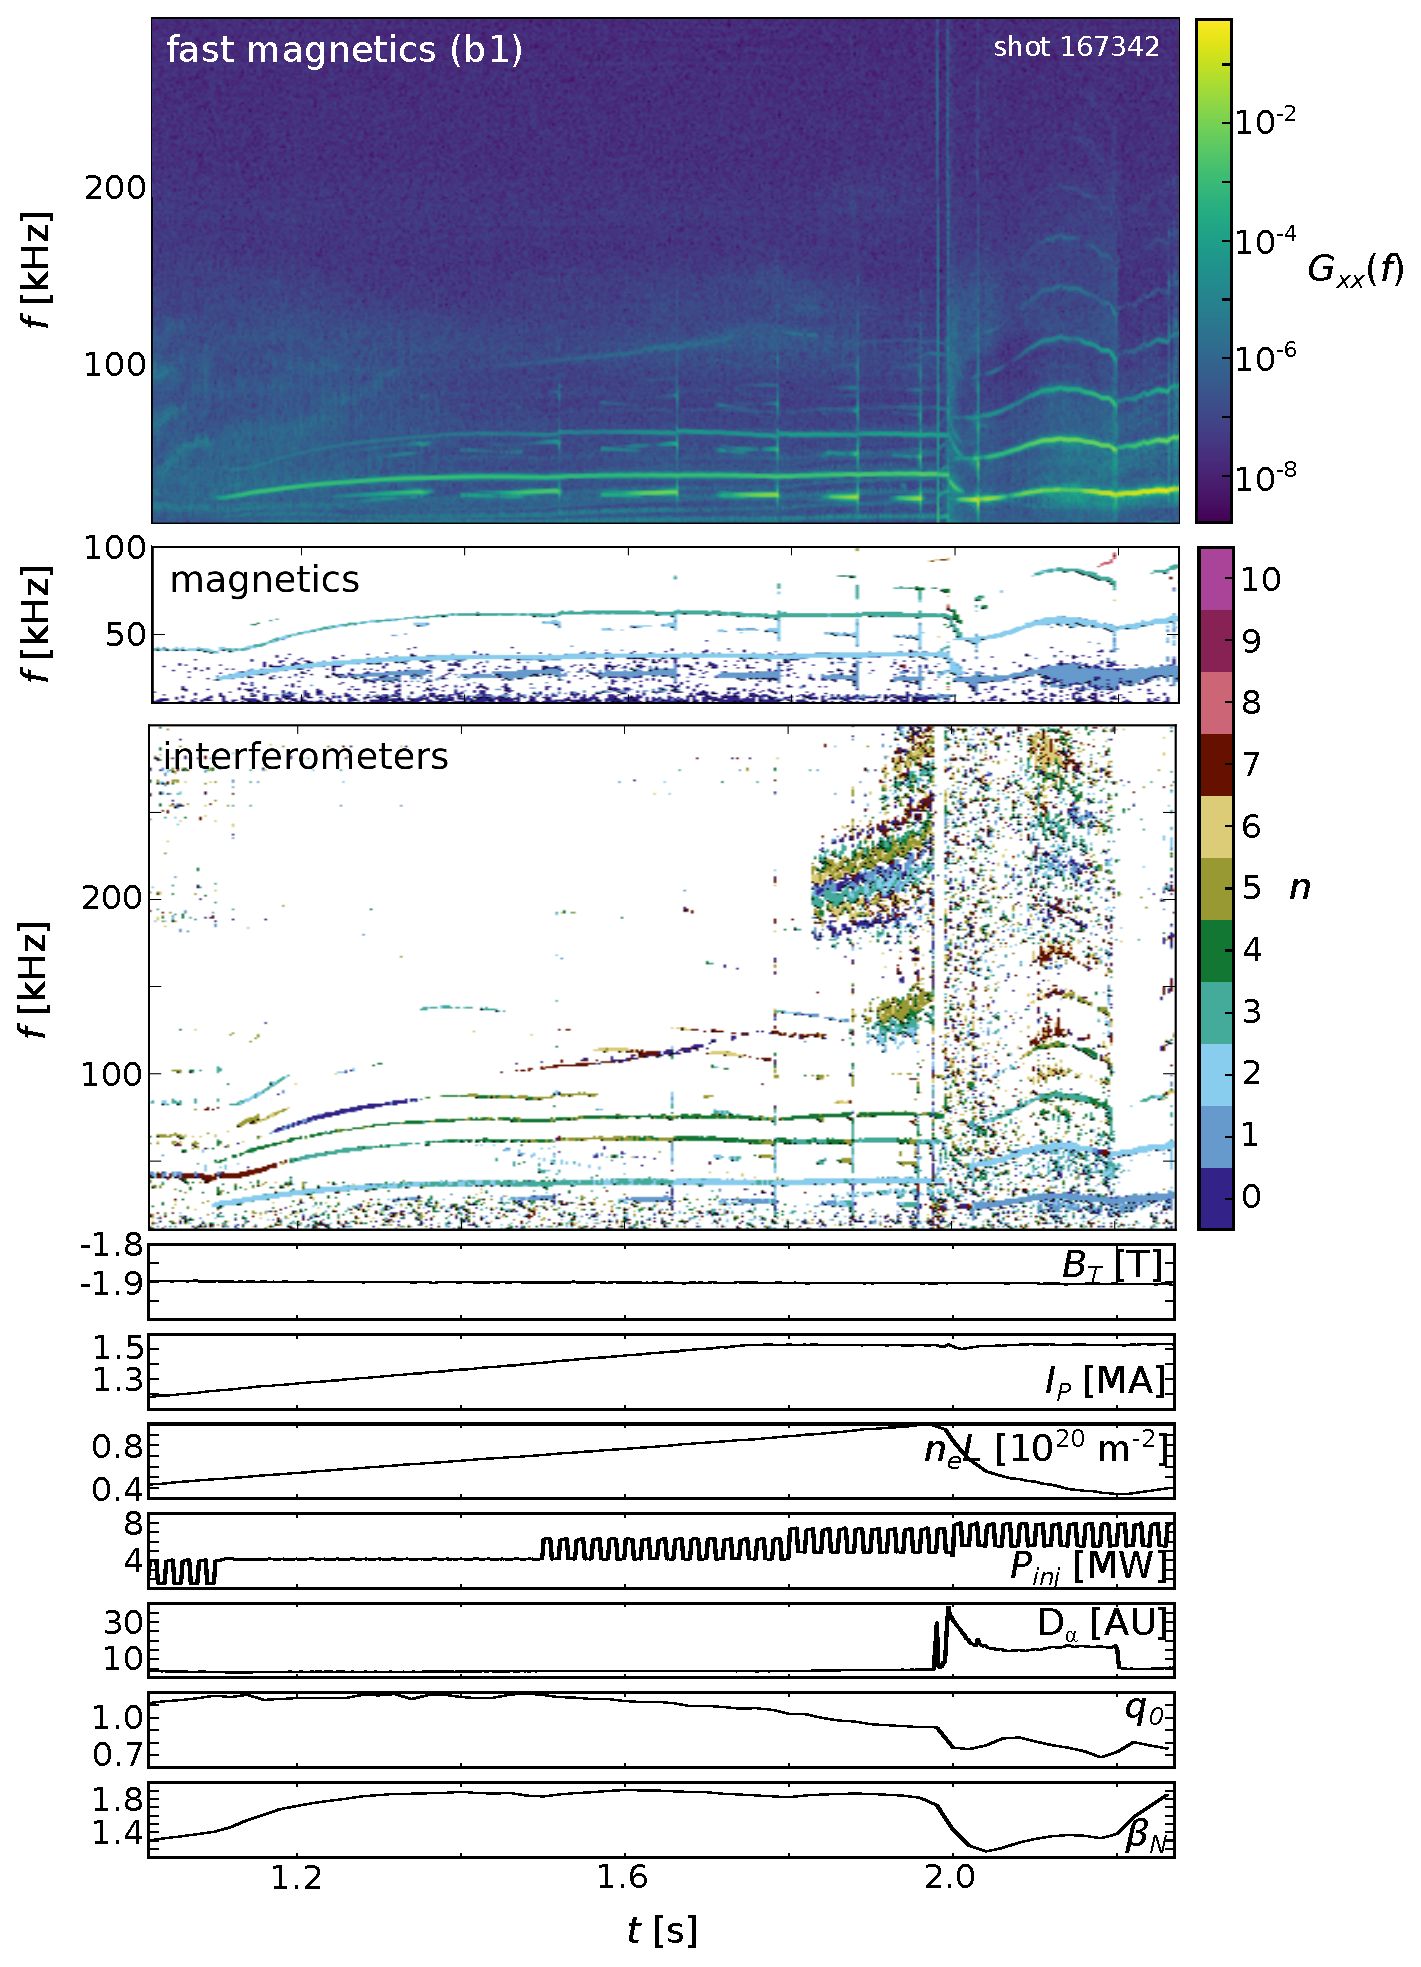
\includegraphics[width = \textwidth]{%
    Chapters/ToroidalCorrelation/figs/core_localized_167342.eps}
  \caption[Toroidal mode numbers of \emph{core-localized} MHD]{%
    Between $\SI{1.8}{\second}$ and $\SI{2.2}{\second}$,
    the correlated interferometers ($3\ts{rd}$ panel) measure
    a burst of fluctuations that are
    \emph{invisible} to magnetics ($1\ts{st}$ and $2\ts{nd}$ panels).
    This suggests that the modes are \emph{core-localized} and
    that the correlated interferometers are indeed capable
    of measuring core-localized MHD.
    Various plasma parameters of interest are shown in the lower panels;
    the modes are triggered when
    the on-axis safety factor $q_0$ drops below unity.
  }
\label{fig:ToroidalCorrelation:core_localized}
\end{figure}


\bibliographystyle{plainurl}
\bibliography{references}
